% Options for packages loaded elsewhere
\PassOptionsToPackage{unicode}{hyperref}
\PassOptionsToPackage{hyphens}{url}
%
\documentclass[
  ignorenonframetext,
]{beamer}
\title{An Introduction to R}
\author{Reio Tanji \and Osaka Univ., Graduate School of Econ.}
\date{April, 2022}

\usepackage{pgfpages}
\setbeamertemplate{caption}[numbered]
\setbeamertemplate{caption label separator}{: }
\setbeamercolor{caption name}{fg=normal text.fg}
\beamertemplatenavigationsymbolsempty
% Prevent slide breaks in the middle of a paragraph
\widowpenalties 1 10000
\raggedbottom
\setbeamertemplate{part page}{
  \centering
  \begin{beamercolorbox}[sep=16pt,center]{part title}
    \usebeamerfont{part title}\insertpart\par
  \end{beamercolorbox}
}
\setbeamertemplate{section page}{
  \centering
  \begin{beamercolorbox}[sep=12pt,center]{part title}
    \usebeamerfont{section title}\insertsection\par
  \end{beamercolorbox}
}
\setbeamertemplate{subsection page}{
  \centering
  \begin{beamercolorbox}[sep=8pt,center]{part title}
    \usebeamerfont{subsection title}\insertsubsection\par
  \end{beamercolorbox}
}
\AtBeginPart{
  \frame{\partpage}
}
\AtBeginSection{
  \ifbibliography
  \else
    \frame{\sectionpage}
  \fi
}
\AtBeginSubsection{
  \frame{\subsectionpage}
}
\usepackage{amsmath,amssymb}
\usepackage{lmodern}
\usepackage{iftex}
\ifPDFTeX
  \usepackage[T1]{fontenc}
  \usepackage[utf8]{inputenc}
  \usepackage{textcomp} % provide euro and other symbols
\else % if luatex or xetex
  \usepackage{unicode-math}
  \defaultfontfeatures{Scale=MatchLowercase}
  \defaultfontfeatures[\rmfamily]{Ligatures=TeX,Scale=1}
\fi
% Use upquote if available, for straight quotes in verbatim environments
\IfFileExists{upquote.sty}{\usepackage{upquote}}{}
\IfFileExists{microtype.sty}{% use microtype if available
  \usepackage[]{microtype}
  \UseMicrotypeSet[protrusion]{basicmath} % disable protrusion for tt fonts
}{}
\makeatletter
\@ifundefined{KOMAClassName}{% if non-KOMA class
  \IfFileExists{parskip.sty}{%
    \usepackage{parskip}
  }{% else
    \setlength{\parindent}{0pt}
    \setlength{\parskip}{6pt plus 2pt minus 1pt}}
}{% if KOMA class
  \KOMAoptions{parskip=half}}
\makeatother
\usepackage{xcolor}
\IfFileExists{xurl.sty}{\usepackage{xurl}}{} % add URL line breaks if available
\IfFileExists{bookmark.sty}{\usepackage{bookmark}}{\usepackage{hyperref}}
\hypersetup{
  pdftitle={An Introduction to R},
  pdfauthor={Reio Tanji; Osaka Univ., Graduate School of Econ.},
  hidelinks,
  pdfcreator={LaTeX via pandoc}}
\urlstyle{same} % disable monospaced font for URLs
\newif\ifbibliography
\usepackage{color}
\usepackage{fancyvrb}
\newcommand{\VerbBar}{|}
\newcommand{\VERB}{\Verb[commandchars=\\\{\}]}
\DefineVerbatimEnvironment{Highlighting}{Verbatim}{commandchars=\\\{\}}
% Add ',fontsize=\small' for more characters per line
\usepackage{framed}
\definecolor{shadecolor}{RGB}{248,248,248}
\newenvironment{Shaded}{\begin{snugshade}}{\end{snugshade}}
\newcommand{\AlertTok}[1]{\textcolor[rgb]{0.94,0.16,0.16}{#1}}
\newcommand{\AnnotationTok}[1]{\textcolor[rgb]{0.56,0.35,0.01}{\textbf{\textit{#1}}}}
\newcommand{\AttributeTok}[1]{\textcolor[rgb]{0.77,0.63,0.00}{#1}}
\newcommand{\BaseNTok}[1]{\textcolor[rgb]{0.00,0.00,0.81}{#1}}
\newcommand{\BuiltInTok}[1]{#1}
\newcommand{\CharTok}[1]{\textcolor[rgb]{0.31,0.60,0.02}{#1}}
\newcommand{\CommentTok}[1]{\textcolor[rgb]{0.56,0.35,0.01}{\textit{#1}}}
\newcommand{\CommentVarTok}[1]{\textcolor[rgb]{0.56,0.35,0.01}{\textbf{\textit{#1}}}}
\newcommand{\ConstantTok}[1]{\textcolor[rgb]{0.00,0.00,0.00}{#1}}
\newcommand{\ControlFlowTok}[1]{\textcolor[rgb]{0.13,0.29,0.53}{\textbf{#1}}}
\newcommand{\DataTypeTok}[1]{\textcolor[rgb]{0.13,0.29,0.53}{#1}}
\newcommand{\DecValTok}[1]{\textcolor[rgb]{0.00,0.00,0.81}{#1}}
\newcommand{\DocumentationTok}[1]{\textcolor[rgb]{0.56,0.35,0.01}{\textbf{\textit{#1}}}}
\newcommand{\ErrorTok}[1]{\textcolor[rgb]{0.64,0.00,0.00}{\textbf{#1}}}
\newcommand{\ExtensionTok}[1]{#1}
\newcommand{\FloatTok}[1]{\textcolor[rgb]{0.00,0.00,0.81}{#1}}
\newcommand{\FunctionTok}[1]{\textcolor[rgb]{0.00,0.00,0.00}{#1}}
\newcommand{\ImportTok}[1]{#1}
\newcommand{\InformationTok}[1]{\textcolor[rgb]{0.56,0.35,0.01}{\textbf{\textit{#1}}}}
\newcommand{\KeywordTok}[1]{\textcolor[rgb]{0.13,0.29,0.53}{\textbf{#1}}}
\newcommand{\NormalTok}[1]{#1}
\newcommand{\OperatorTok}[1]{\textcolor[rgb]{0.81,0.36,0.00}{\textbf{#1}}}
\newcommand{\OtherTok}[1]{\textcolor[rgb]{0.56,0.35,0.01}{#1}}
\newcommand{\PreprocessorTok}[1]{\textcolor[rgb]{0.56,0.35,0.01}{\textit{#1}}}
\newcommand{\RegionMarkerTok}[1]{#1}
\newcommand{\SpecialCharTok}[1]{\textcolor[rgb]{0.00,0.00,0.00}{#1}}
\newcommand{\SpecialStringTok}[1]{\textcolor[rgb]{0.31,0.60,0.02}{#1}}
\newcommand{\StringTok}[1]{\textcolor[rgb]{0.31,0.60,0.02}{#1}}
\newcommand{\VariableTok}[1]{\textcolor[rgb]{0.00,0.00,0.00}{#1}}
\newcommand{\VerbatimStringTok}[1]{\textcolor[rgb]{0.31,0.60,0.02}{#1}}
\newcommand{\WarningTok}[1]{\textcolor[rgb]{0.56,0.35,0.01}{\textbf{\textit{#1}}}}
\setlength{\emergencystretch}{3em} % prevent overfull lines
\providecommand{\tightlist}{%
  \setlength{\itemsep}{0pt}\setlength{\parskip}{0pt}}
\setcounter{secnumdepth}{-\maxdimen} % remove section numbering
\ifLuaTeX
  \usepackage{selnolig}  % disable illegal ligatures
\fi

\begin{document}
\frame{\titlepage}

\begin{frame}{はじめに}
\protect\hypertarget{ux306fux3058ux3081ux306b}{}
\begin{itemize}
\tightlist
\item
  このスライドはhtml形式で保存しています

  \begin{itemize}
  \tightlist
  \item
    左下のハンバーガーアイコンをクリックすると各ページに飛べます
  \item
    ただ、PC以外の方法で閲覧するのはちょっと不便
  \end{itemize}
\item
  ファイルをpdfで保存することができます

  \begin{itemize}
  \tightlist
  \item
    ブラウザURLの末尾に''?print-pdf''を付け、ページを印刷するとpdf形式で保存できます
  \item
    紙に印刷して見たい、単純に見づらいからpdfで閲覧したいという方はどうぞ
  \end{itemize}
\end{itemize}
\end{frame}

\begin{frame}[fragile]{R言語を使う}
\protect\hypertarget{rux8a00ux8a9eux3092ux4f7fux3046}{}
\begin{itemize}
\tightlist
\item
  R言語とは?
\item
  Rでできること

  \begin{itemize}
  \tightlist
  \item
    研究・分析のフロー
  \end{itemize}
\item
  R言語の基本構造
\end{itemize}

\begin{block}{R言語とは?}
\protect\hypertarget{rux8a00ux8a9eux3068ux306f}{}
\begin{itemize}
\item
  ``\emph{R is a free software environment for statistical computing and
  graphics}''(from \href{https://www.r-project.org/}{The R Project for
  Statistical Computing})

  \begin{itemize}
  \tightlist
  \item
    統計計算、グラフ作成を行うことができる無料のツール
  \item
    データの収集、管理、分析から結果の出力・プレゼンテーションの作成までを一つの言語で行うことも出来る
  \item
    この資料もRを使って作成(R Markdown)
  \end{itemize}
\item
  目標

  \begin{itemize}
  \tightlist
  \item
    今回は、Rの基本的な操作方法を学習した上で、論文執筆の上で最低限必要なアウトプットのための技術習得をめざす
  \end{itemize}
\end{itemize}
\end{block}

\begin{block}{Rでできること}
\protect\hypertarget{rux3067ux3067ux304dux308bux3053ux3068}{}
\begin{itemize}
\item
  データの操作

  \begin{itemize}
  \tightlist
  \item
    データの取得:デフォルトのデータセット、csvファイル等の読み込み
  \item
    データの整理:必要な情報の抽出、データの変形、新たな変数の作成と保存
  \end{itemize}
\item
  データの要約・可視化

  \begin{itemize}
  \tightlist
  \item
    基本統計量の作成
  \item
    変数間の関係を視覚的に描写:graphics, ggplot2
  \end{itemize}
\item
  データ分析

  \begin{itemize}
  \tightlist
  \item
    計量経済学・統計学で用いられる様々な手法の実装
  \item
    結果の出力
  \end{itemize}
\item
  レポートの作成

  \begin{itemize}
  \item
    分析結果をスライドにして報告 RMarkdown

    \begin{itemize}
    \tightlist
    \item
      Word, Powerpoint形式でファイルを出力
    \end{itemize}
  \item
    出力の保存や体裁を整える手間が削減できる
  \end{itemize}
\end{itemize}
\end{block}

\begin{block}{データの操作}
\protect\hypertarget{ux30c7ux30fcux30bfux306eux64cdux4f5c}{}
\begin{itemize}
\tightlist
\item
  利用するデータの読み込み
\end{itemize}

\begin{center}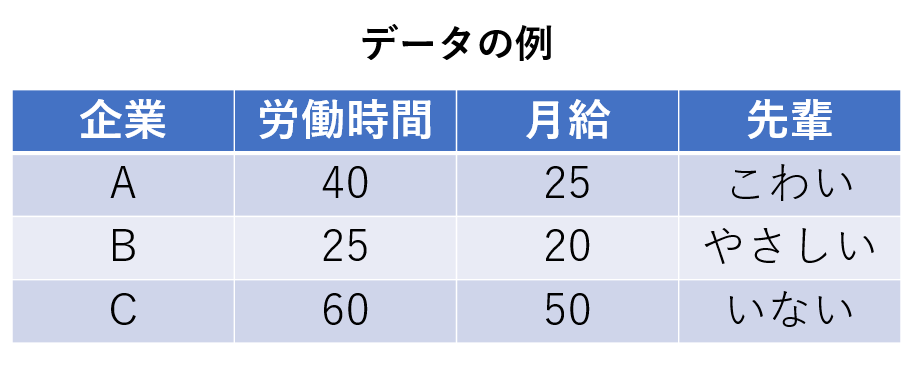
\includegraphics[width=0.7\linewidth]{figs/data_rei} \end{center}

\begin{itemize}
\item
  データを加工する

  \begin{itemize}
  \tightlist
  \item
    欲しい行だけ抜き出す、欲しい列だけ抜き出す
  \item
    元データの情報を使って、分析のための新しい変数を作る
  \item
    例えば、人口50万人以上の都市に1,
    それ以外に0を入れる「大都市ダミー」を作成する
  \end{itemize}
\end{itemize}
\end{block}

\begin{block}{データの要約・可視化}
\protect\hypertarget{ux30c7ux30fcux30bfux306eux8981ux7d04ux53efux8996ux5316}{}
\begin{itemize}
\tightlist
\item
  要約統計量の作成
\end{itemize}

\begin{center}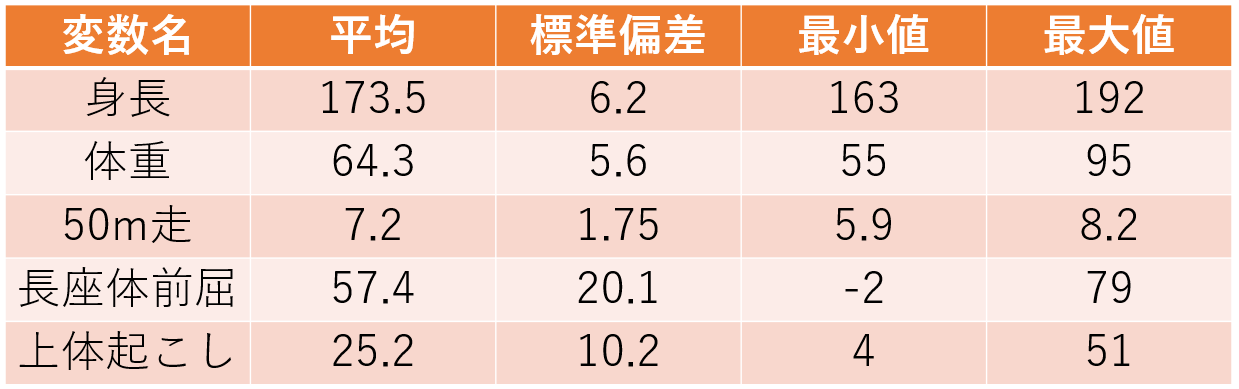
\includegraphics[width=0.8\linewidth]{figs/summary_ex} \end{center}

\begin{itemize}
\tightlist
\item
  データの概要を示す:各変数の平均・標準偏差など
\item
  性別ごと、年代ごとなど、カテゴリで分けて表示する場合も
\item
  可視化できるデータは可視化すると分かりやすい
\end{itemize}
\end{block}

\begin{block}{可視化されたデータの例}
\protect\hypertarget{ux53efux8996ux5316ux3055ux308cux305fux30c7ux30fcux30bfux306eux4f8b}{}
\begin{Shaded}
\begin{Highlighting}[]
\NormalTok{df }\OtherTok{\textless{}{-}}\NormalTok{ palmerpenguins}\SpecialCharTok{::}\NormalTok{penguins}
\NormalTok{ggplot2}\SpecialCharTok{::}\FunctionTok{ggplot}\NormalTok{(df) }\SpecialCharTok{+}
\NormalTok{  ggplot2}\SpecialCharTok{::}\FunctionTok{aes}\NormalTok{(}\AttributeTok{x =}\NormalTok{ body\_mass\_g, }\AttributeTok{y =}\NormalTok{ bill\_length\_mm, }\AttributeTok{colour =}\NormalTok{ species) }\SpecialCharTok{+}
\NormalTok{  ggplot2}\SpecialCharTok{::}\FunctionTok{geom\_point}\NormalTok{() }\SpecialCharTok{+}
\NormalTok{  ggplot2}\SpecialCharTok{::}\FunctionTok{scale\_colour\_viridis\_d}\NormalTok{()}
\end{Highlighting}
\end{Shaded}

\begin{center}\includegraphics{introduction1_files/figure-beamer/unnamed-chunk-3-1} \end{center}
\end{block}

\begin{block}{データ分析}
\protect\hypertarget{ux30c7ux30fcux30bfux5206ux6790}{}
\begin{itemize}
\tightlist
\item
  回帰分析などの統計手法による分析を行い、結果をまとめる
\end{itemize}

\[\text{weight}_{i} = \text{flipperSize}_i + \text{Spiecies}_i + u_i\]

\begin{verbatim}
## 
## Call:
## lm(formula = body_mass_g ~ flipper_length_mm + species, data = .)
## 
## Residuals:
##     Min      1Q  Median      3Q     Max 
## -927.70 -254.82  -23.92  241.16 1191.68 
## 
## Coefficients:
##                    Estimate Std. Error t value Pr(>|t|)    
## (Intercept)       -4031.477    584.151  -6.901 2.55e-11 ***
## flipper_length_mm    40.705      3.071  13.255  < 2e-16 ***
## speciesChinstrap   -206.510     57.731  -3.577 0.000398 ***
## speciesGentoo       266.810     95.264   2.801 0.005392 ** 
## ---
## Signif. codes:  0 '***' 0.001 '**' 0.01 '*' 0.05 '.' 0.1 ' ' 1
## 
## Residual standard error: 375.5 on 338 degrees of freedom
##   ( 2 個の観測値が欠損のため削除されました )
## Multiple R-squared:  0.7826, Adjusted R-squared:  0.7807 
## F-statistic: 405.7 on 3 and 338 DF,  p-value: < 2.2e-16
\end{verbatim}
\end{block}

\begin{block}{レポートの作成}
\protect\hypertarget{ux30ecux30ddux30fcux30c8ux306eux4f5cux6210}{}
\begin{itemize}
\tightlist
\item
  Rで行った分析の結果を、Wordやパワーポイントにまとめて出力、保存できる
\item
  習熟度によってはそのまま論文を書くことも可能、そこまでいかずとも色々と手間が省けて便利
\end{itemize}
\end{block}

\begin{block}{おまけ:データの取得}
\protect\hypertarget{ux304aux307eux3051ux30c7ux30fcux30bfux306eux53d6ux5f97}{}
\begin{itemize}
\tightlist
\item
  Rでは様々なデータセットを
\item
  ウェブサイトから情報を収集して分析を行いたい場合がある
\item
  Rのコードからウェブサイトを開き、中の要素を分析に使えるデータセットとして出力することができる
\end{itemize}
\end{block}

\begin{block}{基本構造}
\protect\hypertarget{ux57faux672cux69cbux9020}{}
\begin{itemize}
\item
  基本的には、というか全ての命令は

  \begin{itemize}
  \item
    Rに命令を投げる→命令に従って計算(描画・読み込みなど)を行う
  \item
    必要であればアウトプットを返す
  \end{itemize}

  の繰り返し
\item
  エレベーターの3階ボタンを押す→3階に向かう、ドアを開ける

  \begin{itemize}
  \tightlist
  \item
    ボタンを押すエネルギーでエレベータが動いているわけではない
  \item
    ワイヤーをどれだけ巻き取ればどれだけ上昇・下降するのか、ドアを開けるためにどの部分にどれだけ力を加えればいいのか、が3回ボタンを押したときに発せられる命令として書かれている
  \end{itemize}
\item
  この命令を一つ一つ書く作業を行う
\end{itemize}
\end{block}

\begin{block}{参考}
\protect\hypertarget{ux53c2ux8003}{}
\begin{itemize}
\tightlist
\item
  立命館大:森先生のサイトが大変勉強になります

  \begin{itemize}
  \tightlist
  \item
    \href{https://tomoecon.github.io/R_for_graduate_thesis/}{卒業論文のためのR入門}
  \end{itemize}
\item
  その他、分からないことはgoogleする力を付けましょう

  \begin{itemize}
  \tightlist
  \item
    ``r (関数名)''とかで大体載ってます
  \item
    GitHubなどで自身の作成したライブラリや関数の使い方などを解説しているものも多数存在
  \end{itemize}
\item
  \href{http://cse.naro.affrc.go.jp/takezawa/r-tips/r.html}{R Tips}
\item
  \href{http://www.okadajp.org/RWiki/}{RjpWiki}
\end{itemize}
\end{block}

\begin{block}{その他}
\protect\hypertarget{ux305dux306eux4ed6}{}
\begin{itemize}
\tightlist
\item
  ショートカット:マウスを極力使わない→作業効率の改善
\item
  共通の操作

  \begin{itemize}
  \tightlist
  \item
    Ctrl + X, C, V:順に切り取り・コピー・貼り付け
  \item
    Ctrl + A:全範囲を選択
  \item
    Ctrl + Z, Y:操作を戻す・進める
  \item
    Ctrl + F:ウィンドウ内検索
  \item
    Ctrl + S:(上書き)保存
  \end{itemize}
\item
  R Studio内の操作

  \begin{itemize}
  \tightlist
  \item
    Ctrl + Shift + N:新しいスクリプトを開く
  \item
    Ctrl + O:保存したファイルを開く(Studio以外でもだいたい使える)
  \item
    Ctrl + W:タブを閉じる(Chromeとかブラウザも同じ)
  \item
    Ctrl + Q:R Studioの終了
  \end{itemize}
\item
  Word, PowerPoint, Excelを扱うときもできるだけマウスを使わない

  \begin{itemize}
  \tightlist
  \item
    慣れると作業効率がだいぶ変わる
  \end{itemize}
\end{itemize}
\end{block}
\end{frame}

\begin{frame}[fragile]{Setup}
\protect\hypertarget{setup}{}
\begin{itemize}
\tightlist
\item
  Rでの作業に使うもの

  \begin{itemize}
  \tightlist
  \item
    開発環境とは、R Studioのすすめ
  \end{itemize}
\item
  インストール
\item
  基本操作画面
\end{itemize}

\begin{block}{Rでの作業に必要なもの}
\protect\hypertarget{rux3067ux306eux4f5cux696dux306bux5fc5ux8981ux306aux3082ux306e}{}
\begin{itemize}
\tightlist
\item
  \textbf{R言語}と\textbf{R Studio}の2つをインストール

  \begin{itemize}
  \tightlist
  \item
    R言語をスムーズに利用するためのツール:開発環境がRStudio
  \item
    デフォルトでR GUI
    と呼ばれる開発環境がインストールされるが、色々な理由から使いづらい

    \begin{itemize}
    \tightlist
    \item
      罫線の引いてあるノートに書くか、自由帳に書くかみたいな違い
    \item
      最終的にR言語で命令を書くのは同じ
    \end{itemize}
  \item
    その他にも Jupyter Notebook, VS Code,
    Atomなど様々な開発環境があるので、好きなものを使えばよい
  \end{itemize}
\item
  R Studio Cloud: クラウド上でR Studioの機能を利用できるサービス

  \begin{itemize}
  \tightlist
  \item
    無料の場合は月あたりの利用時間が制限されるなど問題はあるが、特に自前PCのない人は検討してみてもよいかも
  \end{itemize}
\end{itemize}
\end{block}

\begin{block}{RとR Studio}
\protect\hypertarget{rux3068r-studio}{}
\begin{center}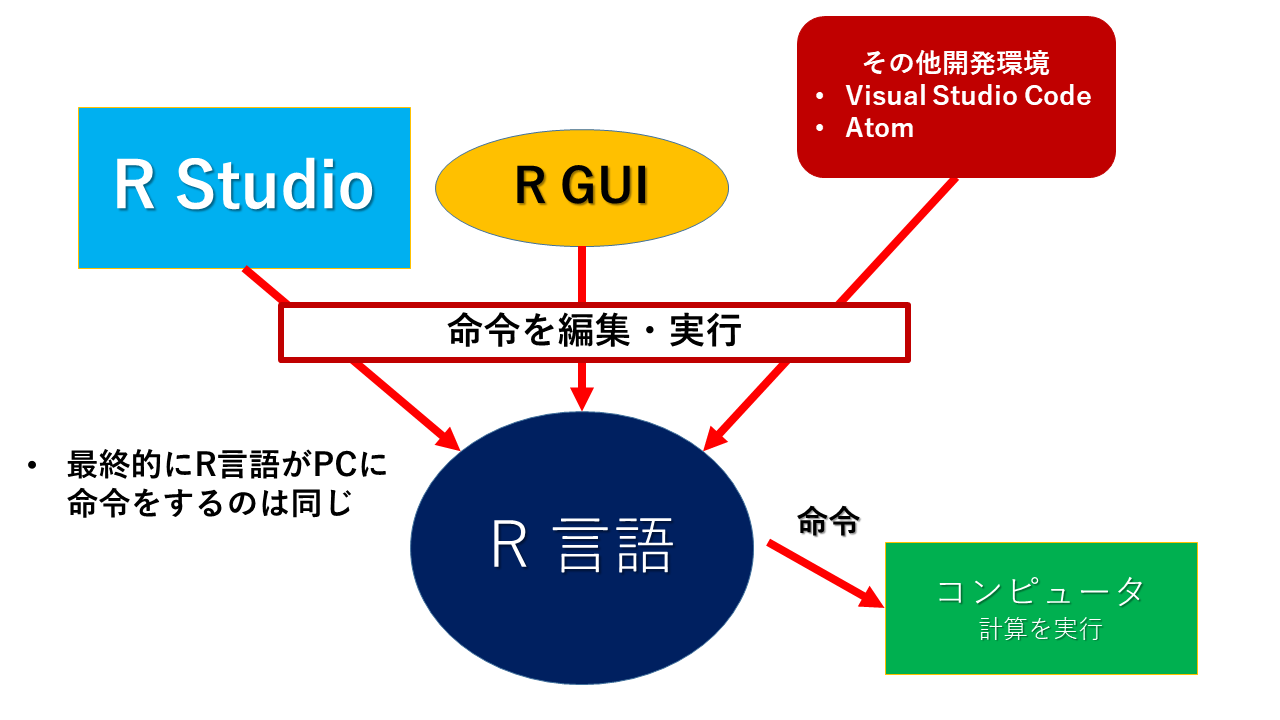
\includegraphics[width=0.95\linewidth]{figs/r_structure} \end{center}
\end{block}

\begin{block}{CSVファイルと Microsoft Excel}
\protect\hypertarget{csvux30d5ux30a1ux30a4ux30ebux3068-microsoft-excel}{}
\begin{itemize}
\tightlist
\item
  csvファイル:データをカンマ(,)と改行を使って表現するテキストデータ

  \begin{itemize}
  \tightlist
  \item
    Officeが入っているPCでは、拡張子「.csv」のファイルはExcelで開かれるが、別にExcel以外では使えないわけではない
  \end{itemize}
\item
  これを一般的なテキストエディタで開くとこうなる
\end{itemize}
\end{block}

\begin{block}{インストール}
\protect\hypertarget{ux30a4ux30f3ux30b9ux30c8ux30fcux30eb}{}
\href{https://cran.ism.ac.jp/}{Rのダウンロードはここから}

\href{https://www.rstudio.com/products/rstudio/download/\#download}{RStudio
Desktop}

\begin{itemize}
\tightlist
\item
  【定期】詰まったら4回生に訊いて下さい
\item
  それぞれ必ず最新バージョンをダウンロードすること

  \begin{itemize}
  \tightlist
  \item
    定期的にアップデートしておくのがおすすめ、たまに関数の仕様とかが大幅に変わる
  \item
    たぶんいないと思いますが、Ver.4.0.0以前のものを使用している4回生はインストールし直して下さい
  \end{itemize}
\item
  Cドライブに日本語フォントが含まれている人

  \begin{itemize}
  \tightlist
  \item
    C:/Users/\ldots/\ldots のところ
  \item
    ファイルの保存などする際に非常に面倒なことになります
  \item
    特に動作で問題が出なければいいですが、コードの実行中に止まるなどあれば相談して下さい
  \item
    今から買う人は絶対に日本語フォントを入れないようにしましょう、一生
  \end{itemize}
\end{itemize}
\end{block}

\begin{block}{R Studioの基本画面}
\protect\hypertarget{r-studioux306eux57faux672cux753bux9762}{}
\begin{itemize}
\tightlist
\item
  4つの画面 (Pane)が表示される: コードを入力するのは Source,
  Consoleの2つ

  \begin{itemize}
  \tightlist
  \item
    Source:Rスクリプトなどを編集・保存
  \item
    Console:実行するコードを直接入力・実行できる。
  \item
    右側の Pane
    では読み込んだデータフレームやオブジェクトの定義確認、図表出力のチェックなどが行える
  \end{itemize}
\end{itemize}

\begin{center}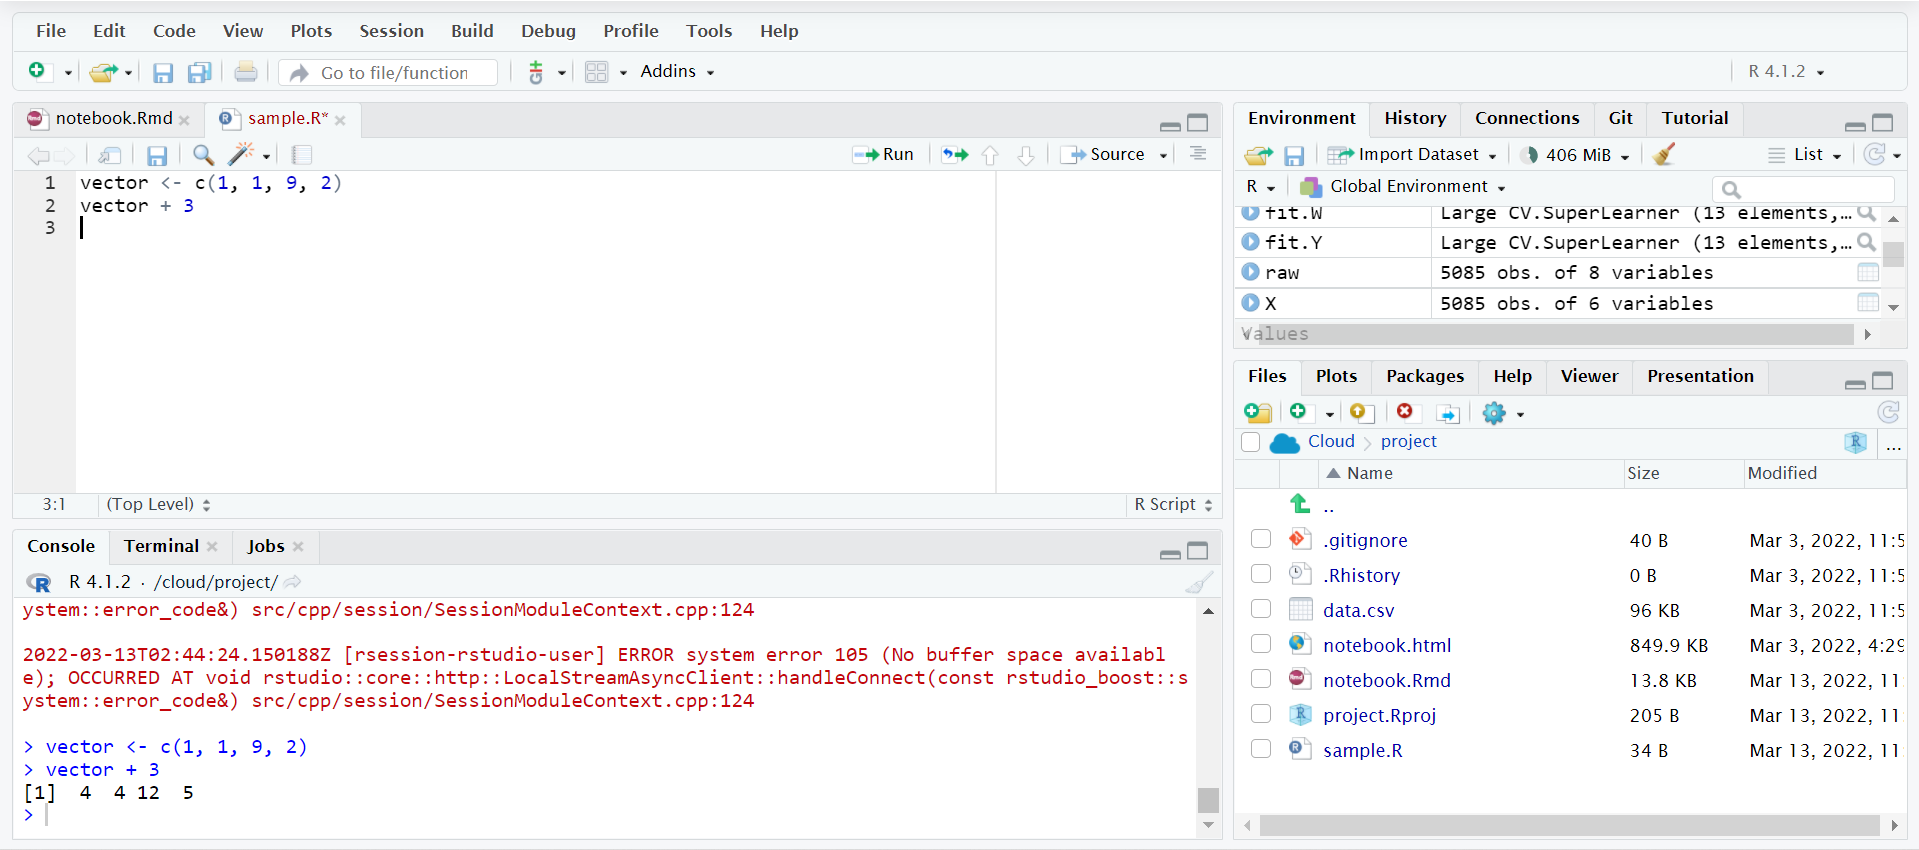
\includegraphics[width=0.77\linewidth]{figs/rstudio_appearance} \end{center}
\end{block}

\begin{block}{触ってみる}
\protect\hypertarget{ux89e6ux3063ux3066ux307fux308b}{}
\begin{itemize}
\tightlist
\item
  コンソールに適当なコードを入力してみよう
\end{itemize}

\begin{Shaded}
\begin{Highlighting}[]
\DecValTok{1} \SpecialCharTok{+} \DecValTok{3} \SpecialCharTok{+} \DecValTok{5}
\end{Highlighting}
\end{Shaded}

\begin{verbatim}
## [1] 9
\end{verbatim}

\begin{itemize}
\tightlist
\item
  コンソールではEnter, ソース(スクリプト)ではCtrl +
  Enterでコードを実行する
\item
  出力は\textgreater に続いて出る(文字色が変わるので分かりやすいはず)
\item
  このスライド上では、コード、出力を四角囲みで、うち出力を\#\#に続く形で表現する
\end{itemize}
\end{block}
\end{frame}

\begin{frame}{プロジェクトの作成、バージョン管理}
\protect\hypertarget{ux30d7ux30edux30b8ux30a7ux30afux30c8ux306eux4f5cux6210ux30d0ux30fcux30b8ux30e7ux30f3ux7ba1ux7406}{}
\begin{itemize}
\tightlist
\item
  ディレクトリとは
\item
  ディレクトリの構造
\item
  フォルダの共有方法
\item
  R Studioでプロジェクトを作成する方法
\end{itemize}

\begin{block}{ディレクトリ}
\protect\hypertarget{ux30c7ux30a3ux30ecux30afux30c8ux30ea}{}
\begin{itemize}
\tightlist
\item
  ファイルやフォルダを参照する際に示すPC内の\textbf{住所}

  \begin{itemize}
  \tightlist
  \item
    C:/\ldots がそれ
  \item
    全てが同じ階層に入っているのは作業こそ楽だが、自分で参照するときに探すのが面倒

    \begin{itemize}
    \tightlist
    \item
      ゼミ論文に使うdata.csvというファイルを保存→他の講義で同じ名前のファイルを受け取る→後から見たらどれがどれだか分からなくなる
    \end{itemize}
  \end{itemize}
\item
  整理の方法:
  作業やファイルの種類ごとにフォルダを作り、異なる系統のファイルを識別

  \begin{itemize}
  \tightlist
  \item
    何をする作業のフォルダなのか?
  \item
    データの種類:整理する前の生データなのか、そのまま分析に使えるデータなのか?
  \item
    アウトプット: 分析結果、図表
  \end{itemize}
\item
  R
  Studioでは、特定のフォルダを「プロジェクト」として扱い、「誰のPCでも動くコード」を作ることができる
\end{itemize}
\end{block}

\begin{block}{ディレクトリの構造}
\protect\hypertarget{ux30c7ux30a3ux30ecux30afux30c8ux30eaux306eux69cbux9020}{}
\begin{center}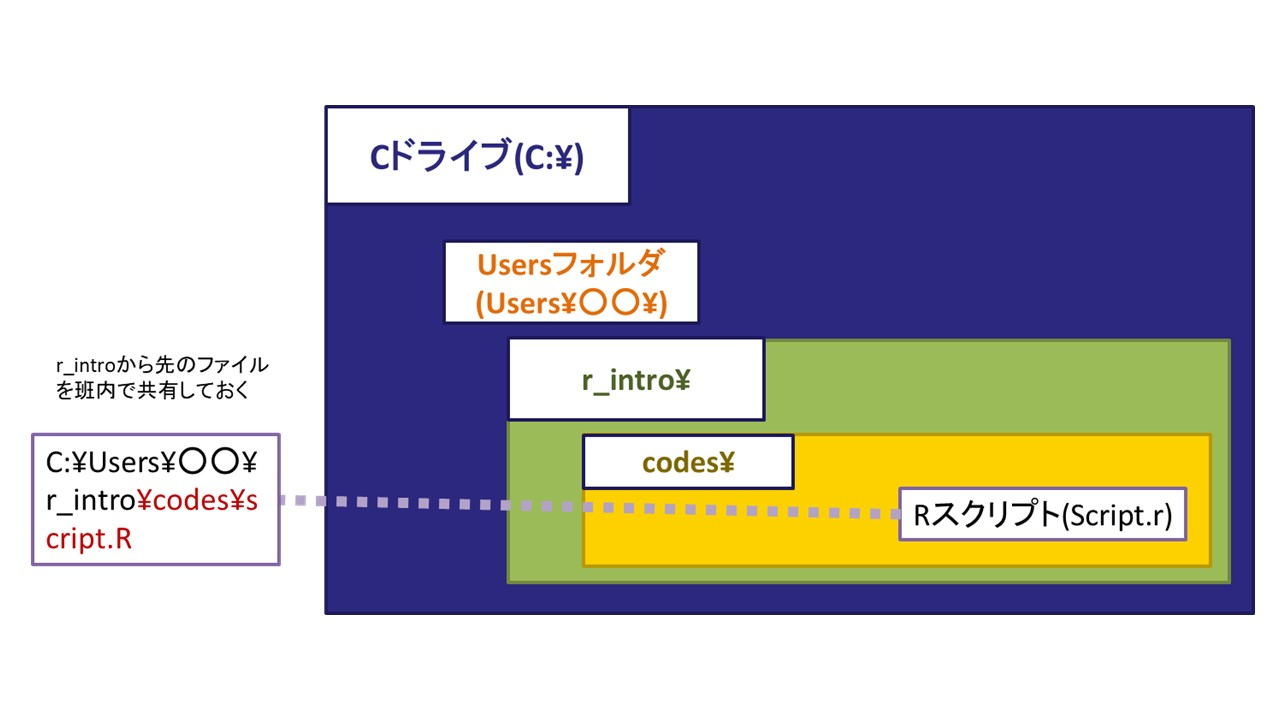
\includegraphics[width=0.77\linewidth]{figs/folder} \end{center}

\begin{itemize}
\tightlist
\item
  使いやすいフォルダの作成

  \begin{itemize}
  \tightlist
  \item
    各自のPCで''r\_intro''フォルダを作り、必要なファイルをしまっておけば、誰が書いたコードでも個々人がPCで再現できる環境に
  \item
    フォルダ名は\textbackslash(バックスラッシュ, ¥)を/
    (スラッシュ)に変えて記述
  \end{itemize}
\end{itemize}
\end{block}

\begin{block}{フォルダ}
\protect\hypertarget{ux30d5ux30a9ux30ebux30c0}{}
\begin{center}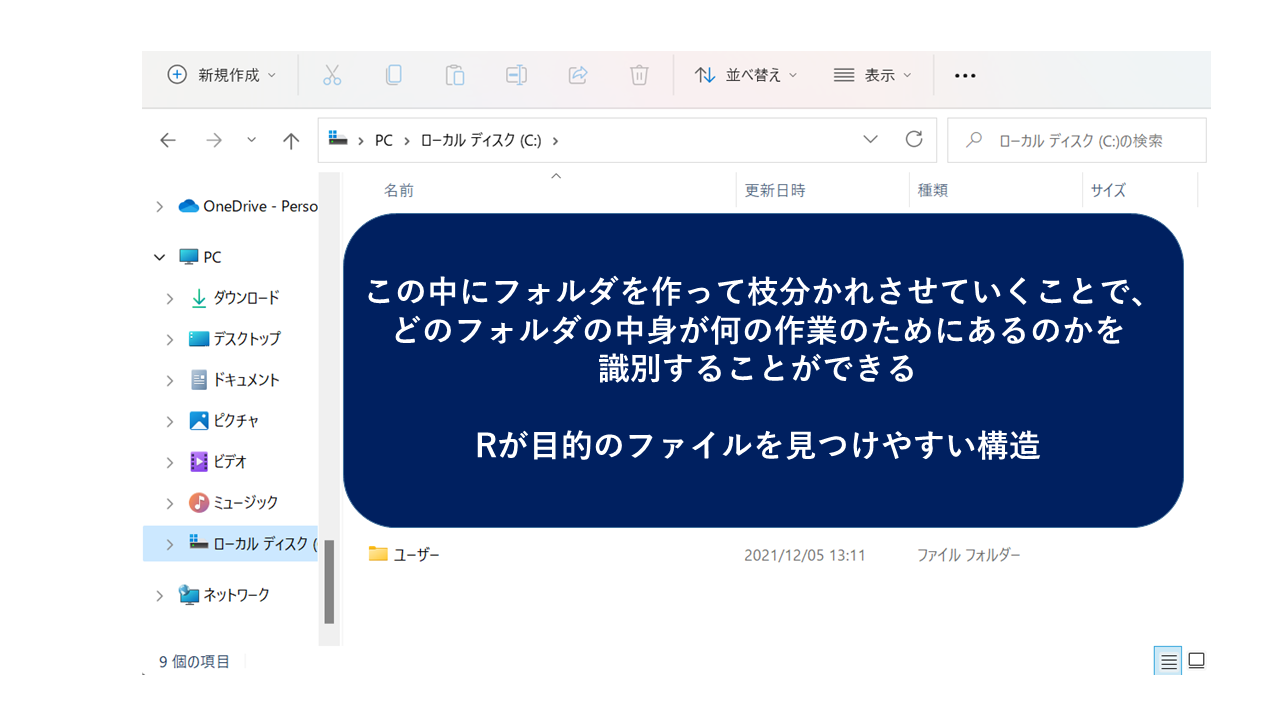
\includegraphics[width=0.95\linewidth]{figs/directory_system} \end{center}
\end{block}

\begin{block}{フォルダ (cont'd)}
\protect\hypertarget{ux30d5ux30a9ux30ebux30c0-contd}{}
\begin{center}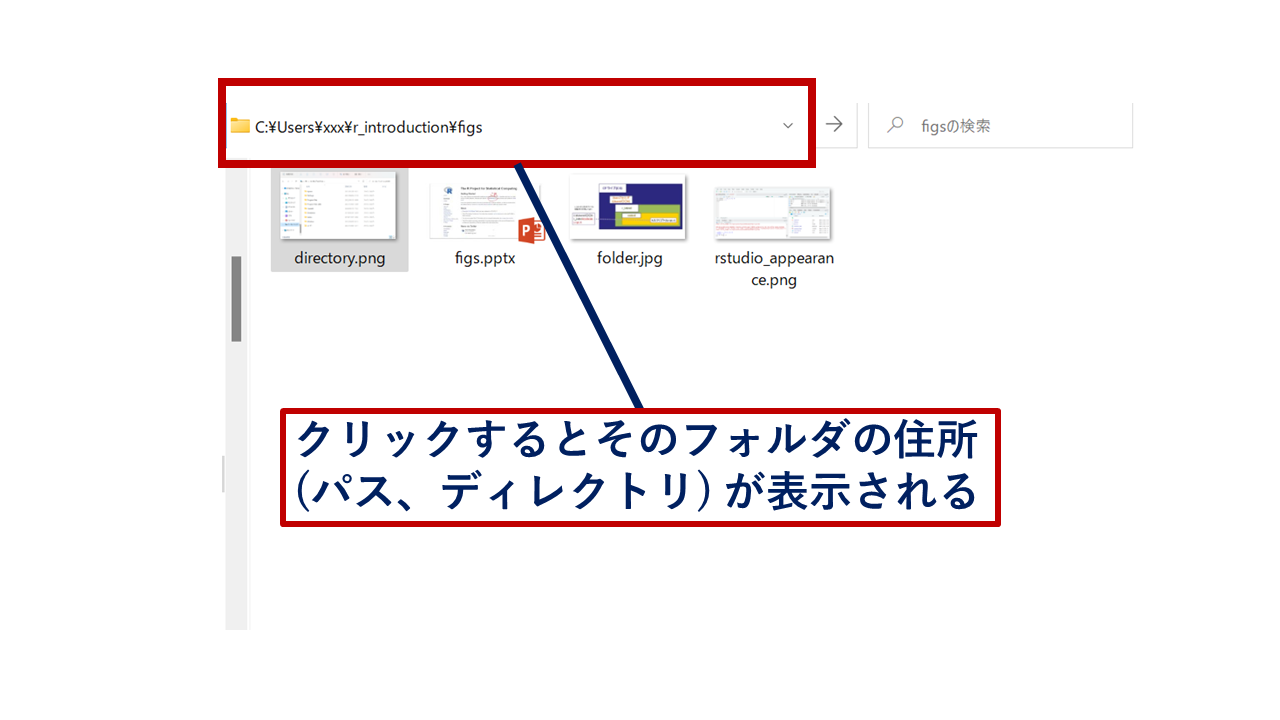
\includegraphics[width=0.95\linewidth]{figs/directory_system2} \end{center}
\end{block}

\begin{block}{拡張子}
\protect\hypertarget{ux62e1ux5f35ux5b50}{}
\begin{itemize}
\tightlist
\item
  PC上で扱うファイルには、それがどのアプリケーション(ソフト)で利用するものなのかがPC側に伝わる印が付いていることが多い:拡張子

  \begin{itemize}
  \tightlist
  \item
    例えば.csvはMicrosoft Excelで開くと決めている(既定のアプリ)
  \item
    .RはRスクリプトを表すことが分かるのでR StudioやR
    GUI、.htmlはブラウザで開く
  \end{itemize}
\end{itemize}
\end{block}

\begin{block}{フォルダの共有方法}
\protect\hypertarget{ux30d5ux30a9ux30ebux30c0ux306eux5171ux6709ux65b9ux6cd5}{}
\begin{itemize}
\tightlist
\item
  フォルダの共有:データや書いたスクリプトを共有する

  \begin{itemize}
  \tightlist
  \item
    何度も修正を加えたり、作った図表を共有するのはめんどい
  \item
    結果、分析をした人がスライドも全部作る\ldots になりがち
  \end{itemize}
\item
  フォルダをメンバー間で同期する(共有する)ツールをマスターすると、グループでの作業が楽になる

  \begin{itemize}
  \tightlist
  \item
    \href{https://www.dropbox.com/}{Dropbox}
  \item
    \href{https://github.com/}{GitHub}
  \end{itemize}
\item
  特にGitHubはRStudioと直接連携して簡単にクラウド共有・共有したデータのダウンロードも可能なので非常に便利

  \begin{itemize}
  \tightlist
  \item
    データをオープンで保有することになるので、扱うデータの種類によっては注意が必要
  \end{itemize}
\end{itemize}
\end{block}

\begin{block}{フォルダの共有方法(cont'd)}
\protect\hypertarget{ux30d5ux30a9ux30ebux30c0ux306eux5171ux6709ux65b9ux6cd5contd}{}
\begin{itemize}
\tightlist
\item
  Google Driveを使う方法もあり

  \begin{itemize}
  \tightlist
  \item
    Google Document, Spreadsheet, Slides を使った論文共同執筆はべんり
  \item
    OfficeのWord, Excel, Powerpointに比べると機能がかなり制限される弱点
  \item
    特にスライド作成に関しては不便なポイントが多いかも
  \end{itemize}
\item
  文面はGoogle
  Driveで共有しながら作成しつつ、体裁を適宜Wordにダウンロードするなどして修正する必要がある
\end{itemize}
\end{block}

\begin{block}{プロジェクトの作り方}
\protect\hypertarget{ux30d7ux30edux30b8ux30a7ux30afux30c8ux306eux4f5cux308aux65b9}{}
\begin{center}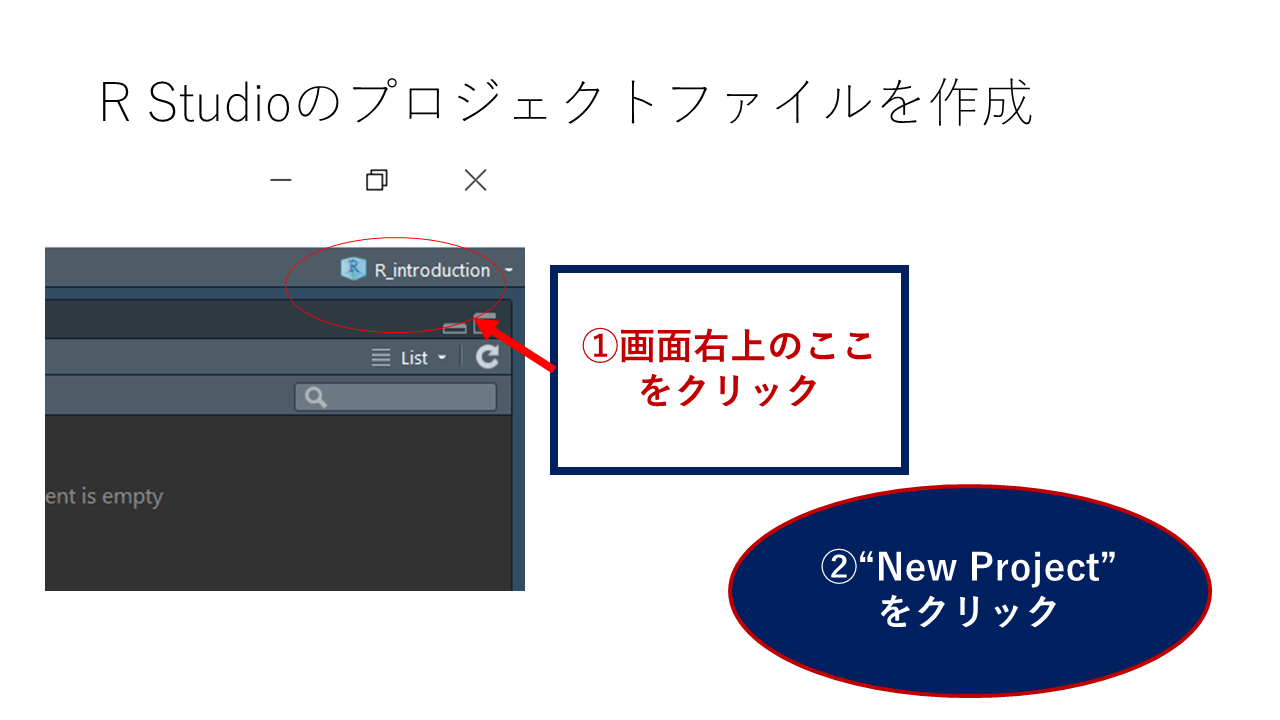
\includegraphics[width=0.95\linewidth]{figs/create_repository} \end{center}
\end{block}

\begin{block}{プロジェクトの作り方(cont'd)}
\protect\hypertarget{ux30d7ux30edux30b8ux30a7ux30afux30c8ux306eux4f5cux308aux65b9contd}{}
\begin{center}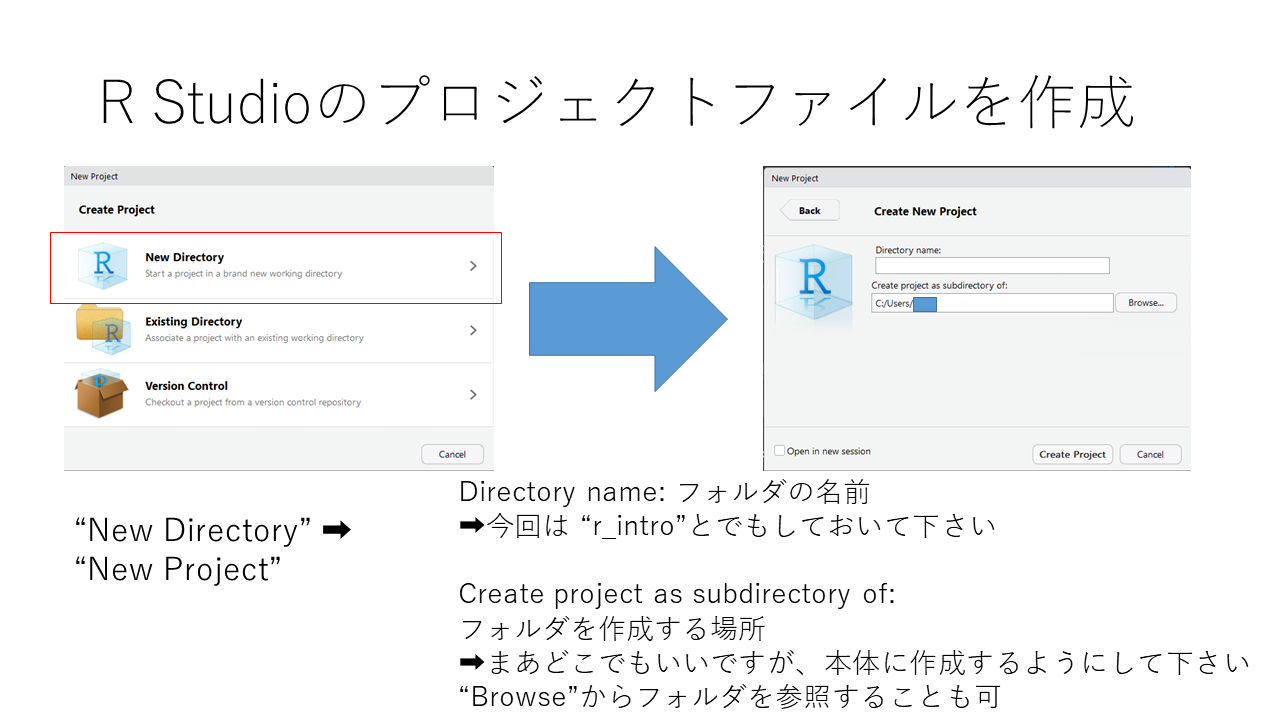
\includegraphics[width=0.95\linewidth]{figs/create_repository2} \end{center}
\end{block}
\end{frame}

\begin{frame}[fragile]{基本操作}
\protect\hypertarget{ux57faux672cux64cdux4f5c}{}
\begin{itemize}
\tightlist
\item
  コンソールに数値を打ち込む、計算する
\item
  スクリプトの作成
\item
  変数の型
\item
  オブジェクトに数値などを割り当てる
\item
  値を束にして扱う
\end{itemize}

\begin{block}{スクリプトの作成、演算子}
\protect\hypertarget{ux30b9ux30afux30eaux30d7ux30c8ux306eux4f5cux6210ux6f14ux7b97ux5b50}{}
\begin{itemize}
\item
  ``r\_introduction''というプロジェクトを作成
\item
  R Studioを開く

  \begin{itemize}
  \tightlist
  \item
    R
    Consoleにコードを直接入力してEnter、もしくはRスクリプトにコードを記述してCtrl
    + Enterで実行
  \item
    RスクリプトはCtrl+Shift+Nで作成可能
  \item
    Ctrl + Sで保存、上書き保存
  \end{itemize}
\end{itemize}

\begin{Shaded}
\begin{Highlighting}[]
\DecValTok{1} \SpecialCharTok{+} \DecValTok{2} \SpecialCharTok{*}\NormalTok{ (}\DecValTok{3} \SpecialCharTok{/} \DecValTok{4}\NormalTok{) }\CommentTok{\# 掛け算は*で}
\end{Highlighting}
\end{Shaded}

\begin{verbatim}
## [1] 2.5
\end{verbatim}

\begin{itemize}
\tightlist
\item
  その他、基本的な演算記号は\href{http://cse.naro.affrc.go.jp/takezawa/r-tips/r.html}{R-Tips}などを参照
\end{itemize}
\end{block}

\begin{block}{変数の型}
\protect\hypertarget{ux5909ux6570ux306eux578b}{}
\begin{itemize}
\tightlist
\item
  数値だけでなく、文字も扱うことができる

  \begin{itemize}
  \tightlist
  \item
    何を使っても良いわけではない:Excelも一緒

    \begin{itemize}
    \tightlist
    \item
      電話番号を入力したのに頭の0が消える→Excelが電話番号を数値として認識してしまっているから
    \item
      Excelの場合、数値の形式を標準(Excelに自己判断させる)から文字列に変更することで対処
    \end{itemize}
  \item
    文字列を''\,``で囲って表記することで、それが文字列であることをRに伝えることができる
  \item
    class関数(関数については後述)を使うと、その値の型が分かる
  \end{itemize}
\end{itemize}

\begin{Shaded}
\begin{Highlighting}[]
\FunctionTok{class}\NormalTok{(}\FloatTok{3.14}\NormalTok{) }\CommentTok{\# class()はその変数の型を返す関数}
\end{Highlighting}
\end{Shaded}

\begin{verbatim}
## [1] "numeric"
\end{verbatim}

\begin{Shaded}
\begin{Highlighting}[]
\FunctionTok{class}\NormalTok{(}\StringTok{\textquotesingle{}1.90\textquotesingle{}}\NormalTok{) }\CommentTok{\# 文字列 character と判定される}
\end{Highlighting}
\end{Shaded}

\begin{verbatim}
## [1] "character"
\end{verbatim}
\end{block}

\begin{block}{変数の型(cont'd)}
\protect\hypertarget{ux5909ux6570ux306eux578bcontd}{}
\begin{itemize}
\tightlist
\item
  numeric, integerは足し引きできるが、characterはできない

  \begin{itemize}
  \tightlist
  \item
    integerは整数
  \end{itemize}
\end{itemize}

\begin{Shaded}
\begin{Highlighting}[]
\StringTok{"1"} \SpecialCharTok{+} \StringTok{"2"} \CommentTok{\# エラーが出る}
\end{Highlighting}
\end{Shaded}

\begin{Shaded}
\begin{Highlighting}[]
\FunctionTok{class}\NormalTok{(11L) }\CommentTok{\# 整数の後ろに"L"を付けると整数として認識される}
\end{Highlighting}
\end{Shaded}

\begin{verbatim}
## [1] "integer"
\end{verbatim}
\end{block}

\begin{block}{変数の型(cont'd)}
\protect\hypertarget{ux5909ux6570ux306eux578bcontd-1}{}
\begin{itemize}
\tightlist
\item
  factor

  \begin{itemize}
  \tightlist
  \item
    順序が付いた文字列
  \item
    factor()で定義
  \item
    アルファベット順や数字順以外の方法で並べたい場合に使う
  \item
    まあ使うときにやればいいとおもいます
  \end{itemize}
\end{itemize}

\begin{Shaded}
\begin{Highlighting}[]
\FunctionTok{factor}\NormalTok{(}\FunctionTok{c}\NormalTok{(}\StringTok{"January"}\NormalTok{, }\StringTok{"February"}\NormalTok{, }\StringTok{"March"}\NormalTok{, }\StringTok{"April"}\NormalTok{)) }\CommentTok{\# アルファベット順に並んでしまう}
\end{Highlighting}
\end{Shaded}

\begin{verbatim}
## [1] January  February March    April   
## Levels: April February January March
\end{verbatim}

\begin{Shaded}
\begin{Highlighting}[]
\FunctionTok{factor}\NormalTok{(}\FunctionTok{c}\NormalTok{(}\StringTok{"January"}\NormalTok{, }\StringTok{"February"}\NormalTok{, }\StringTok{"March"}\NormalTok{, }\StringTok{"April"}\NormalTok{), }
       \AttributeTok{levels =} \FunctionTok{c}\NormalTok{(}\StringTok{"January"}\NormalTok{, }\StringTok{"February"}\NormalTok{, }\StringTok{"March"}\NormalTok{, }\StringTok{"April"}\NormalTok{))}
\end{Highlighting}
\end{Shaded}

\begin{verbatim}
## [1] January  February March    April   
## Levels: January February March April
\end{verbatim}
\end{block}

\begin{block}{オブジェクト}
\protect\hypertarget{ux30aaux30d6ux30b8ux30a7ux30afux30c8}{}
\begin{itemize}
\tightlist
\item
  では''\,``で囲わずに入力した文字列はどう認識されるのか?

  \begin{enumerate}
  \tightlist
  \item
    特定の値と結びついている
  \end{enumerate}

  \begin{itemize}
  \tightlist
  \item
    \texttt{pi}: 円周率
  \end{itemize}

  \begin{enumerate}
  \setcounter{enumi}{1}
  \tightlist
  \item
    自信が定義した任意の値が格納されている
  \end{enumerate}

  \begin{itemize}
  \tightlist
  \item
    オブジェクト: 数値やベクトル、データフレームやリストを格納、R
    Studioでは右上のEnvironmentタブに定義が表示される
  \item
    回帰分析などの計算結果を格納することも可能
  \item
    \texttt{\textless{}-} を使って適当な値を定義する
  \item
    \texttt{wani\ \textless{}-\ 3}:waniというオブジェクトに値3を格納
  \end{itemize}
\item
  R Studioでは Environmentに定義したオブジェクトの中身が表示される
\end{itemize}
\end{block}

\begin{block}{オブジェクトの定義}
\protect\hypertarget{ux30aaux30d6ux30b8ux30a7ux30afux30c8ux306eux5b9aux7fa9}{}
\begin{Shaded}
\begin{Highlighting}[]
\NormalTok{pi }\CommentTok{\# デフォルトで円周率が格納されている}
\end{Highlighting}
\end{Shaded}

\begin{verbatim}
## [1] 3.141593
\end{verbatim}

\begin{Shaded}
\begin{Highlighting}[]
\NormalTok{value }\OtherTok{\textless{}{-}} \DecValTok{8} \CommentTok{\# valueという文字列に8を代入}
\NormalTok{value }\SpecialCharTok{+} \DecValTok{10} \CommentTok{\# 今valueの値は8なので、8 + 10を計算した結果を返してくれる}
\end{Highlighting}
\end{Shaded}

\begin{verbatim}
## [1] 18
\end{verbatim}
\end{block}

\begin{block}{値を束にして扱う}
\protect\hypertarget{ux5024ux3092ux675fux306bux3057ux3066ux6271ux3046}{}
\begin{itemize}
\tightlist
\item
  \(5 \times 5\)なら電卓でやればよい
\item
\end{itemize}
\end{block}

\begin{block}{ベクトル}
\protect\hypertarget{ux30d9ux30afux30c8ux30eb}{}
\begin{itemize}
\tightlist
\item
  ベクトル:複数の要素を含む列

  \begin{itemize}
  \tightlist
  \item
    \texttt{c(a,\ b,\ c,\ ...)}で定義される
  \item
    文字列など、他の数値型を利用してもOK
  \end{itemize}
\end{itemize}

\begin{Shaded}
\begin{Highlighting}[]
\NormalTok{vec }\OtherTok{\textless{}{-}} \FunctionTok{c}\NormalTok{(}\DecValTok{1192}\NormalTok{, }\DecValTok{2960}\NormalTok{)}
\NormalTok{vec }\SpecialCharTok{*} \DecValTok{2}
\end{Highlighting}
\end{Shaded}

\begin{verbatim}
## [1] 2384 5920
\end{verbatim}

\begin{itemize}
\tightlist
\item
  関数(後述)を用いて規則性のあるベクトルを簡単に定義することもできる

  \begin{itemize}
  \tightlist
  \item
    \texttt{seq(a,\ b,\ c)}: aからbまで、公差cの等差数列

    \begin{itemize}
    \tightlist
    \item
      公差が1の場合は、\texttt{a:b}でも代替可能
    \end{itemize}
  \item
    \texttt{rep(a,\ b)}: aをb回繰り返す数列
  \end{itemize}
\end{itemize}

\begin{Shaded}
\begin{Highlighting}[]
\FunctionTok{seq}\NormalTok{(}\DecValTok{1}\NormalTok{, }\DecValTok{10}\NormalTok{, }\DecValTok{2}\NormalTok{)}
\end{Highlighting}
\end{Shaded}

\begin{verbatim}
## [1] 1 3 5 7 9
\end{verbatim}
\end{block}

\begin{block}{データフレーム}
\protect\hypertarget{ux30c7ux30fcux30bfux30d5ux30ecux30fcux30e0}{}
\begin{itemize}
\item
  各行に観測単位(個人、グループ、都道府県など)、各列に特定の情報を含んだデータ形式

  \begin{itemize}
  \tightlist
  \item
    実際にデータ分析を行う際は、csvファイルなどをこの形式で読み込むことでRで扱えるようにする
  \end{itemize}
\item
  100人の性別、学年、学部が分かるデータフレーム:100行×3列のデータフレームになる
\item
  データフレームは\texttt{data.frame}関数、もしくはtibbleパッケージの\texttt{tibble}関数で定義する
\end{itemize}
\end{block}

\begin{block}{データフレーム (cont'd)}
\protect\hypertarget{ux30c7ux30fcux30bfux30d5ux30ecux30fcux30e0-contd}{}
\begin{Shaded}
\begin{Highlighting}[]
\FunctionTok{library}\NormalTok{(tidyverse) }\CommentTok{\# パッケージを起動}
\end{Highlighting}
\end{Shaded}

\begin{Shaded}
\begin{Highlighting}[]
\NormalTok{df }\OtherTok{\textless{}{-}}\NormalTok{ tibble}\SpecialCharTok{::}\FunctionTok{tibble}\NormalTok{( }\CommentTok{\# dfというオブジェクトにデータフレームを定義}
  \AttributeTok{faculty =} \FunctionTok{c}\NormalTok{(}\StringTok{"econ"}\NormalTok{, }\StringTok{"law"}\NormalTok{, }\StringTok{"foreign"}\NormalTok{, }\StringTok{"lit"}\NormalTok{), }\CommentTok{\# 各列のデータをベクトル形式で代入}
  \AttributeTok{grade =} \FunctionTok{c}\NormalTok{(}\DecValTok{4}\NormalTok{, }\DecValTok{2}\NormalTok{, }\DecValTok{1}\NormalTok{, }\DecValTok{1}\NormalTok{),}
  \AttributeTok{toeic =} \FunctionTok{c}\NormalTok{(}\DecValTok{300}\NormalTok{, }\DecValTok{820}\NormalTok{, }\ConstantTok{NA}\NormalTok{, }\DecValTok{785}\NormalTok{) }\CommentTok{\# NA: 該当する値が存在しないことを表す=無回答など}
\NormalTok{)}
\FunctionTok{print}\NormalTok{(df)}
\end{Highlighting}
\end{Shaded}

\begin{verbatim}
## # A tibble: 4 x 3
##   faculty grade toeic
##   <chr>   <dbl> <dbl>
## 1 econ        4   300
## 2 law         2   820
## 3 foreign     1    NA
## 4 lit         1   785
\end{verbatim}
\end{block}

\begin{block}{リスト}
\protect\hypertarget{ux30eaux30b9ux30c8}{}
\begin{itemize}
\tightlist
\item
  値、ベクトル、データフレームなど、何を入れてもいい箱
\item
  \texttt{list(要素1,\ 要素2,\ ...)}で定義
\item
  複数のデータフレームに対して同じ操作をしたい場合などに便利
\end{itemize}

\begin{Shaded}
\begin{Highlighting}[]
\NormalTok{listA }\OtherTok{\textless{}{-}} \FunctionTok{list}\NormalTok{(}\FunctionTok{data.frame}\NormalTok{(}\AttributeTok{a =} \DecValTok{1}\SpecialCharTok{:}\DecValTok{5}\NormalTok{, }\AttributeTok{b =} \DecValTok{11}\SpecialCharTok{:}\DecValTok{15}\NormalTok{, }\AttributeTok{c =} \DecValTok{100}\SpecialCharTok{:}\DecValTok{104}\NormalTok{), df)}
\FunctionTok{print}\NormalTok{(listA)}
\end{Highlighting}
\end{Shaded}

\begin{verbatim}
## [[1]]
##   a  b   c
## 1 1 11 100
## 2 2 12 101
## 3 3 13 102
## 4 4 14 103
## 5 5 15 104
## 
## [[2]]
## # A tibble: 4 x 3
##   faculty grade toeic
##   <chr>   <dbl> <dbl>
## 1 econ        4   300
## 2 law         2   820
## 3 foreign     1    NA
## 4 lit         1   785
\end{verbatim}
\end{block}

\begin{block}{リスト (cont'd)}
\protect\hypertarget{ux30eaux30b9ux30c8-contd}{}
\begin{Shaded}
\begin{Highlighting}[]
\FunctionTok{print}\NormalTok{(listA[[}\DecValTok{1}\NormalTok{]]) }\CommentTok{\# リストの中の一部の要素のみ利用する場合は、[[]]で指定する}
\end{Highlighting}
\end{Shaded}

\begin{verbatim}
##   a  b   c
## 1 1 11 100
## 2 2 12 101
## 3 3 13 102
## 4 4 14 103
## 5 5 15 104
\end{verbatim}

\begin{itemize}
\tightlist
\item
  あんまり便利さが伝わらなさそうなので分析パートで後述
\end{itemize}
\end{block}

\begin{block}{関数}
\protect\hypertarget{ux95a2ux6570}{}
\begin{itemize}
\tightlist
\item
  Rで行う典型的な操作・計算を行う命令
\item
  操作を実行する対象となる値や、実行にあたって選択可能な様々なオプションを(関数名)(引数1
  = ., 引数2 = ., \ldots)の形で記述
\end{itemize}

\begin{Shaded}
\begin{Highlighting}[]
\FunctionTok{log}\NormalTok{(}\AttributeTok{x =} \DecValTok{100}\NormalTok{, }\AttributeTok{base =} \DecValTok{10}\NormalTok{) }\CommentTok{\# 100の対数、底10で計算}
\end{Highlighting}
\end{Shaded}

\begin{verbatim}
## [1] 2
\end{verbatim}

\begin{Shaded}
\begin{Highlighting}[]
\FunctionTok{log}\NormalTok{(}\AttributeTok{x =} \DecValTok{100}\NormalTok{, }\AttributeTok{base =} \DecValTok{5}\NormalTok{) }\CommentTok{\# 底を5に変更}
\end{Highlighting}
\end{Shaded}

\begin{verbatim}
## [1] 2.861353
\end{verbatim}

\begin{itemize}
\tightlist
\item
  デフォルトで搭載されている関数の他に、便利な関数をまとめて利用可能にする「パッケージ」をインストール・活用することもできる
\end{itemize}

\begin{Shaded}
\begin{Highlighting}[]
\FunctionTok{install.packages}\NormalTok{(}\StringTok{"tidyverse"}\NormalTok{) }\CommentTok{\# tidyverse パッケージをインストール}
\FunctionTok{library}\NormalTok{(tidyverse) }\CommentTok{\# tidyverse パッケージを有効化:起動したときに毎回実行する}
\end{Highlighting}
\end{Shaded}
\end{block}

\begin{block}{関数 (cont'd)}
\protect\hypertarget{ux95a2ux6570-contd}{}
\begin{itemize}
\tightlist
\item
  各関数において使用される引数の名前は決まっており、必要なオプションに対して一つひとつ情報を指定する

  \begin{itemize}
  \tightlist
  \item
    引数には数値や文字列を取ったり、ベクトルやデータフレームを取る時もある
  \end{itemize}
\item
  引数を指定しなければエラーが出るものと、指定しない場合のオプションを自動で選んでくれるものとが存在
\item
  パッケージ名::関数名()でその関数がどのパッケージに属しているかを明示することもできる
\item
  実行結果のエラー

  \begin{itemize}
  \tightlist
  \item
    エラー:引数指定の不備などで計算が実行できなかった場合
  \item
    警告(warning):引数を自動補完した、計算結果に不備があるなどしたが、とりあえず結果は出た
  \end{itemize}
\end{itemize}
\end{block}

\begin{block}{例:図形の描画}
\protect\hypertarget{ux4f8bux56f3ux5f62ux306eux63cfux753b}{}
\begin{itemize}
\tightlist
\item
  \(y = x^2\)のグラフの描画、定義域は-5から5
\item
  pchはプロットの形を指定、colはプロットの色
\end{itemize}

\begin{Shaded}
\begin{Highlighting}[]
\NormalTok{graphics}\SpecialCharTok{::}\FunctionTok{plot}\NormalTok{(}\AttributeTok{x =} \SpecialCharTok{{-}}\DecValTok{5}\SpecialCharTok{:}\DecValTok{5}\NormalTok{, }\AttributeTok{y =}\NormalTok{ (}\SpecialCharTok{{-}}\DecValTok{5}\SpecialCharTok{:}\DecValTok{5}\NormalTok{)}\SpecialCharTok{\^{}}\DecValTok{2}\NormalTok{, }\AttributeTok{pch =} \DecValTok{19}\NormalTok{, }\AttributeTok{col =} \StringTok{"magenta"}\NormalTok{) }
\end{Highlighting}
\end{Shaded}

\begin{center}\includegraphics[width=0.47\linewidth]{introduction1_files/figure-beamer/unnamed-chunk-24-1} \end{center}
\end{block}
\end{frame}

\begin{frame}[fragile]{データの操作}
\protect\hypertarget{ux30c7ux30fcux30bfux306eux64cdux4f5c-1}{}
\begin{itemize}
\tightlist
\item
  デフォルト/特定のパッケージに含まれるデータの利用
\item
  外部ファイルからデータを読み込む
\item
  データの概要を把握する:記述統計の表示
\item
  データを整理する

  \begin{itemize}
  \tightlist
  \item
    新しい変数を作成する
  \item
    不要な行を削除する
  \item
    不要な列を削除する
  \item
    文字列の処理
  \end{itemize}
\end{itemize}

\begin{block}{データの取得}
\protect\hypertarget{ux30c7ux30fcux30bfux306eux53d6ux5f97}{}
\begin{itemize}
\tightlist
\item
  分析方法が決まったらデータを取得
\item
  ここではRで簡単に利用できるサンプルデータを取得して分析・可視化を行う
\item
  palmerpenguinsパッケージをインストール、penguins\_rawデータを使ってみる
\end{itemize}

\begin{Shaded}
\begin{Highlighting}[]
\FunctionTok{install.packages}\NormalTok{(}\StringTok{"palmerpenguins"}\NormalTok{)}
\end{Highlighting}
\end{Shaded}

\begin{itemize}
\tightlist
\item
  パッケージを読み込むとデータセットが利用できるようになる
\end{itemize}

\begin{Shaded}
\begin{Highlighting}[]
\FunctionTok{library}\NormalTok{(palmerpenguins)}
\NormalTok{palmerpenguins}\SpecialCharTok{::}\NormalTok{penguins\_raw}
\end{Highlighting}
\end{Shaded}
\end{block}

\begin{block}{データを確認}
\protect\hypertarget{ux30c7ux30fcux30bfux3092ux78baux8a8d}{}
\includegraphics[width=0.8\linewidth]{introduction1_files/figure-beamer/unnamed-chunk-27-1}
\end{block}

\begin{block}{CSVファイルからデータフレームを読み込み}
\protect\hypertarget{csvux30d5ux30a1ux30a4ux30ebux304bux3089ux30c7ux30fcux30bfux30d5ux30ecux30fcux30e0ux3092ux8aadux307fux8fbcux307f}{}
\begin{itemize}
\tightlist
\item
  csv (comma separated values)
\end{itemize}
\end{block}

\begin{block}{Penguins データの概要}
\protect\hypertarget{penguins-ux30c7ux30fcux30bfux306eux6982ux8981}{}
\begin{itemize}
\tightlist
\item
  ペンギンをとっ捕まえて大きさや重さを計測したデータ
\item
  元論文:\href{https://journals.plos.org/plosone/article?id=10.1371/journal.pone.0090081}{Kristen
  B. Gorman ,Tony D. Williams, and William R. Fraser (2014)}
\item
  論文引用のフォーマット

  \begin{itemize}
  \tightlist
  \item
    Gorman KB, Williams TD, Fraser WR (2014) Ecological Sexual
    Dimorphism and Environmental Variability within a Community of
    Antarctic Penguins (Genus Pygoscelis). PLoS ONE 9(3): e90081.
    {[}\url{https://doi.org/10.1371/journal.pone.0090081}{]}
  \item
    ``Cite''
    みたいなボタンを押すと簡単にフォーマットをコピーできることが多いです
  \end{itemize}
\item
  head(データフレーム, 行数)でデータの行頭を表示させることができる
\end{itemize}

\begin{Shaded}
\begin{Highlighting}[]
\FunctionTok{head}\NormalTok{(penguins\_raw, }\DecValTok{5}\NormalTok{)}
\end{Highlighting}
\end{Shaded}

\begin{verbatim}
## # A tibble: 5 x 17
##   studyName `Sample Number` Species          Region Island Stage `Individual ID`
##   <chr>               <dbl> <chr>            <chr>  <chr>  <chr> <chr>          
## 1 PAL0708                 1 Adelie Penguin ~ Anvers Torge~ Adul~ N1A1           
## 2 PAL0708                 2 Adelie Penguin ~ Anvers Torge~ Adul~ N1A2           
## 3 PAL0708                 3 Adelie Penguin ~ Anvers Torge~ Adul~ N2A1           
## 4 PAL0708                 4 Adelie Penguin ~ Anvers Torge~ Adul~ N2A2           
## 5 PAL0708                 5 Adelie Penguin ~ Anvers Torge~ Adul~ N3A1           
## # ... with 10 more variables: `Clutch Completion` <chr>, `Date Egg` <date>,
## #   `Culmen Length (mm)` <dbl>, `Culmen Depth (mm)` <dbl>,
## #   `Flipper Length (mm)` <dbl>, `Body Mass (g)` <dbl>, Sex <chr>,
## #   `Delta 15 N (o/oo)` <dbl>, `Delta 13 C (o/oo)` <dbl>, Comments <chr>
\end{verbatim}
\end{block}
\end{frame}

\begin{frame}{データの概観:可視化}
\protect\hypertarget{ux30c7ux30fcux30bfux306eux6982ux89b3ux53efux8996ux5316}{}
\begin{itemize}
\tightlist
\item
  データを可視化する:ggplot2パッケージの利用
\end{itemize}
\end{frame}

\begin{frame}{分析と結果の表示}
\protect\hypertarget{ux5206ux6790ux3068ux7d50ux679cux306eux8868ux793a}{}
\begin{itemize}
\tightlist
\item
  分析目的の設定
\item
  最小二乗法
\item
  最尤法

  \begin{itemize}
  \tightlist
  \item
    ロジスティック回帰
  \end{itemize}
\item
  操作変数法
\end{itemize}
\end{frame}

\begin{frame}{RMarkdownを用いたレポートの作成}
\protect\hypertarget{rmarkdownux3092ux7528ux3044ux305fux30ecux30ddux30fcux30c8ux306eux4f5cux6210}{}
\begin{itemize}
\tightlist
\item
  Markdown形式のドキュメント

  \begin{itemize}
  \tightlist
  \item
    数式フォントの利用
  \end{itemize}
\item
  コードブロックの作成
\item
  htmlドキュメントの作成
\item
  Wordファイルへの変換
\item
  Powerpointファイルへの変換
\item
  R Markdownを併用して論文作成・スライド作成の手間を省く
\end{itemize}

\begin{block}{Markdownとは}
\protect\hypertarget{markdownux3068ux306f}{}
\begin{itemize}
\tightlist
\item
  主にhtml(ウェブサイトなどで利用される形式)を手軽に出力するために考案された言語
\item
  Rの結果出力などに特化した形式:R Markdown

  \begin{itemize}
  \tightlist
  \item
    ここではR Markdownについて扱う
  \item
    htmlだけでなく、WordやPowerPointなど、使い慣れた形式にも変換可能
  \end{itemize}
\item
  分析結果をいちいちスクリーンショットしたり、体裁を整えるために出力をやり直したりする必要がなくなる

  \begin{itemize}
  \tightlist
  \item
    全てをR
    Markdownで完結させる必要はないので、例えば図や分析結果の出力をするためのWordファイルを作り、できたものをコピペするなどして使えば微調整も容易
  \end{itemize}
\end{itemize}
\end{block}
\end{frame}

\begin{frame}{おまけ:バージョン管理}
\protect\hypertarget{ux304aux307eux3051ux30d0ux30fcux30b8ux30e7ux30f3ux7ba1ux7406}{}
\begin{itemize}
\tightlist
\item
  論文執筆・輪読の資料報告は班単位で行うので、スライドや分析結果を複数人で作成・共有する必要がある
\item
  Dropbox, Github, Google Drive
  などでファイルごと共有しておくと、スライドをくっつけたり各自が修正したものをすり合わせる作業が削減できる、たぶん
\item
  覚えておいて損はないのでまあ興味があれば訊いて下さい
\end{itemize}
\end{frame}

\end{document}
